\documentclass{article}

\usepackage[brazil]{babel}

\usepackage[letterpaper,top=2cm,bottom=2cm,left=3cm,right=3cm,marginparwidth=1.75cm]{geometry}
\usepackage{amsmath}
\usepackage{graphicx}
\usepackage[colorlinks=true, allcolors=blue]{hyperref}
\usepackage{caption}
\usepackage{float}
\usepackage{csquotes}

\sloppy

\begin{document}

\begin{titlepage}
	\begin{center}
		{\large Universidade Federal de Minas Gerais}\\[0.2cm]
		{\large Instituto de Ciências Exatas}\\[0.2cm]
		{\large Departamento de Ciência da Computação}\\[0.2cm]
		{\large Projeto Final da disciplina de Aprendizado
		Descritivo}\\[5.1cm]
		{\large \bf Mineração de dados de eventos em futebol}\\[5.1cm]
	\end{center}
	{\large Alunos: Luís Felipe Ramos Ferreira, Igor Lacerda Faria da
	Silva,
	Matheus Tiago Pimenta de Souza}\\[0.7cm]
	{\large Professor: Renato Vimieiro}\\[5.1cm]
	\begin{center}
		{\large Belo Horizonte - Minas Gerais}\\[0.2cm]
		{\large 2024}
	\end{center}
\end{titlepage}

\newpage
\begin{quote}
	fala zezé, bom dia cara
\end{quote}

\newpage
\renewcommand{\contentsname}{Sumário}
\tableofcontents
\newpage

\title{Mineração de dados de evento em futebol}
\author{Luís Felipe Ramos Ferreira \\  Igor Lacerda iFaria da Silva \\ Matheus
	Tiago Pimenta de Souza}

\maketitle

\section{Introdução}

O uso de ciência de dados e estatística para analisar esportes é algo que vem
crescendo cada vez mais nos últimos anos. Em
particular, o futebol tem sido um desses
esportes \cite{takvorian2021beautiful}. A própria UFMG ofertou no
ano passado e novamente neste semestre a disciplina ``Ciência de Dados Aplicada
ao Futebol'', o que mostra a relevância do tema. Diversas empresas que atuam na
área surgem a cada dia, e os times de futebol, no Brasil e no resto do
mundo, estão investindo em seus departamentos de dados e estatística.

Nesse sentido, nosso grupo optou por estudar e compreender melhor como funciona
o uso de análises estatísticas no futebol, dado o interesse geral pelo esporte,
e, para isso, nos propusemos a aplicar algoritmos de mineração de dados em
dados futebolísticos, sendo eles dados de súmula, dados de eventos ou até mesmo
dados de
\textit{tracking} dos jogadores, para compreender como as informações acerca do
jogo estão contidas dentro dos dados coletados e como isso pode ser utilizado a
favor das equipes.

Os dados de eventos, especialmente, costumam ser mais fáceis de lidar e mais
fáceis de acessar do que dados de \textit{tracking}, enquanto trazem muito mais
informações do que dados de súmula. Existem, atualmente, algumas bases
gratuitas de dados de evento de partidas, disponibilizadas por diferentes
empresas como \textit{Wyscout} e \textit{StasBomb}. Como a ideia é ter um
panorama geral de diversas partidas, campeonatos e jogadores, iremos utilizar
as bases de dados disponibilizadas sobre as 5 grandes ligas de futebol europeu
das temporadas 17/18 da empresa \textit{Wyscout}.

\subsection{Base de dados}

A principal base disponibilizada pela empresa \textit{Wyscout} foi usada como
nossa base de dados. Ela contém dados de evento das 5 grandes ligas europeias na
temporada 17/18.

Cada empresa fornecedora de dados possui seu próprio formato de representação
dos dados de evento. De modo a facilitar a mesclagem entre as bases de dados
utilizadas, iremos converter os dados coletados para uma representação geral
proposta por pesquisadores denominada
\href{https://socceraction.readthedocs.io/en/latest/documentation/spadl/spadl.html}{SPADL}.
A SPADL é uma boa escolha por ser uma representação concisa e fácil de
utilizar. Ela é uma representação tabular de cada evento da partida, onde cada
linha possui 12 colunas. A tabela abaixo ilustra o esquema de representação de
um evento segundo o formato SPADL.

\begin{table}[H]
	\centering
	\begin{tabular}{|l|l|}
		\hline
		\textbf{Atributo} & \textbf{Descrição}
		\\
		\hline
		game\_id          & O ID do jogo no qual a ação foi realizada
		\\
		\hline
		period\_id        & O ID do período do jogo no qual a ação foi
		realizada
		\\
		\hline
		seconds           & O tempo de início da ação
		\\
		\hline
		player            & O jogador que realizou a ação
		\\
		\hline
		team              & O time do jogador
		\\
		\hline
		start\_x          & A localização x onde a ação começou
		\\
		\hline
		start\_y          & A localização y onde a ação começou
		\\
		\hline
		end\_x            & A localização x onde a ação terminou
		\\
		\hline
		end\_y            & A localização y onde a ação terminou
		\\
		\hline
		action\_type      & O tipo de ação (por exemplo, passe, chute,
		drible)
		\\
		\hline
		result            & O resultado da ação (por exemplo, sucesso
		ou falha)
		\\
		\hline
		bodypart          & A parte do corpo do jogador usada para a
		ação
		\\
		\hline
	\end{tabular}
	\caption{Descrição dos dados no formato SPADL}
\end{table}

\section{Implementação}

A linguagem escolhida para o desenvolvimento do trabalho foi
\href{https://www.python.org/}{\texttt{Python}} (versão 3.10.12), devida a seu
vasto ecossistema para ciência de dados e mineração de dados.

A manipulação dos dados foi feita com o uso de bibliotecas
de análise numérica como \href{https://numpy.org/}{\texttt{NumPy}} e
manipulação de \textit{dataframes} como
\href{https://pola.rs/}{\texttt{Polars}} e
\href{https://pandas.pydata.org/}{\texttt{Pandas}},
uma vez que se tratam de ferramentas extremamente completas que facilitaram o
desenvolvimento do projeto como um todo.

Para aplicar os algoritmos de descobertas de subgrupos, foi utilizado o pacote
\href{https://pysubgroup.readthedocs.io/en/latest/}{\texttt{pysubgroup}}, que
fornece uma aglomeração de algoritmos do estado da arte de descoberta de
subgrupos em um formato simples e leve para serem utilizados.

% falar aq de uqal pacote utilizamos para minerar as sequencias

Para organizar o ambiente de desenvolvimento, que englobava vários pacotes
diferentes, foi utilizado o gerenciador de pacotes
\href{https://www.anaconda.com/}{\texttt{Anaconda}}, o que facilitou o trabalho
com os pacotes de ciência de dados citados. O projeto final foi salvo em um
\href{https://github.com/lframosferreira/projeto-ad}{\texttt{repositório}}
no GitHub para fácil versionamento e organização de código. As instruções de
como utilizar o que foi implementado estão descritas no \textit{README}
do repositório.

\section{Referencial Teórico}

No decorrer do trabalho, duas importantes métricas de análise ofensiva no
futebol serão utilizadas. Esta seção
aglomera os conhecimentos necessários sobre elas para a compreensão do projeto
e o como elas foram utilizadas.

\subsection{Gols Esperados (\textit{xG})}

Intuitivamente, existe a noção de que, quanto mais próximo um jogador está do
gol, mais chance ele tem de conseguir marcar um ponto para sua equipe. Uma
noção similar existe para o ângulo entre o gol e jogador: é mais difícil um
atacante acertar se ele está em uma das laterais. Na área de \textit{analytics}
de futebol, essa noção é formalizada através da métrica de \textit{expected
goals}, ou \textit{xG}. A ideia central é construir um modelo do que um jogador
médio faria em dado estado de jogo, que, além de incluir os fatores mencionados
anteriormente, pode ser mais (ou menos) extensivo.

A métrica de Gols Esperados captura um estado de jogo e retorna uma
probabilidade estimada de um jogador marcar. Ela pode ser vista como um
\textit{framework}, cujos detalhes de implementação são decididos pelo usuário.
Outros fatores considerados importantes são: parte do corpo associada à ação
(pé dominante ou não; de cabeça), origem da assistência (cruzamento, passe) e a
posição dos defensores. Para avaliar este último quesito, é necessário ter
dados de \textit{tracking}, o que limita consideravelmente sua adoção. Além disso,
mesmo questões como a liga em análise podem ser relevantes.

O uso do \textit{xG} é mais amplo do que se pode imaginar a princípio. Em um
primeiro momento, partidas podem ser analisadas: é possível avaliar se um time
fez mais ``pressão'' pela soma do seu \textit{xG} na partida. No entanto, como
com qualquer outro indicador, o \textit{xG} não define absolutamente o
resultado de um jogo, podendo um time aproveitar muito bem situações menos
favoráveis. Outra aplicação é avaliação de jogadores: se um jogador
consistentemente faz gols em situações desfavoráveis, isso é um grande indício
de que ele é jogador de destaque, ou age muito bem sob pressão. O \textit{xG}
também pode ser usado taticamente, para proporcionar melhorias no
posicionamento dos jogadores da \textit{defesa} e para embasar estratégias.

É comum usar modelos de regressão logística para aplicar o \textit{xG}, em que
se considera uma combinação dos fatores mencionados anteriormente. Essa
combinação não é necessariamente linear: considerar o quadrado da distância
pode ser valioso, por exemplo. Na prática, no entanto, qualquer modelo de
classificação binária pode ser usado. Um exemplo muito prevalente é o
\textit{xG} do \textit{Statsbomb}, que usa um \textit{XGBoost} e considera a
quantidade e a posição dos jogadores entre o gol e o jogador que faz o lance.

\subsection{Valuing Actions by Estimating Probabilities (VAEP)}

O \textit{xG} deixa a desejar em alguns aspectos. Principalmente pelo fato de
focar exclusivamente nas chances de se fazer gols, sem considerar outros
aspectos importantes do jogo. Por exemplo, existem passes que são cruciais para
uma equipe se aproximar do gol. É justamente para suprir a necessidade de
avaliar as ações dos jogadores de forma mais ampla que foi desenvolvido o VAEP
\cite{vaep}. O VAEP avalia cada ação do jogo em termos do quanto ela aumenta (ou
diminui) a chance de um time fazer (ou sofrer) um gol.

Com base no estado atual do jogo (placar, tempo restante, ações anteriores,
posição da bola, etc), o VAEP estima a chance de um time fazer ou sofrer um gol,
antes e após cada ação. Desse modo, é possível estimar a utilidade de uma ação
com base na diferença entre as mudanças de se fazer e de se sofrer um gol.
Formalizando, temos que, para um dado time $t$, uma ação $a_i$ e um estado de
jogo $S_i$:

\begin{equation}
	\Delta P_{score}(a_i,t) = P^k_{score}(S_i,t) - P^k_{score}(S_{i-1},t)
	\label{eq:vaep_scores}
\end{equation}

\begin{equation}
	\Delta P_{concede}(a_i,t) = P^k_{concede}(S_i,t) - P^k_{concede}(S_{i-1},t)
	\label{eq:vaep_concedes}
\end{equation}

\begin{equation}
	V_{\textrm{VAEP}}(a_i) = \Delta P_{score}(a_i,t) - \Delta P_{concede}(a_i,t) 
	\label{eq:vaep}
\end{equation}

Nas equações, $k$ é um parâmetro que indica quantas jogadas futuras estão sendo
consideradas para se avaliar a jogada atual. Assim, quando uma jogada aumenta
muito a chance de um gol acontecer, seu VAEP é um número positivo e, caso a
jogada ofereça mais risco do que recompensa, o VAEP será um valor negativo.

Então, para se calcular o VAEP, é necessário estimar as probabilidades de marcar
ou sofrer um gol. Essa tarefa pode ser resolvida com Aprendizado de Máquina, com
a criação de dois modelos: um para estimar a probabilidade da equipe com a posse
da bola fazer um gol até as $k$ ações após o estado atual $S_i$ e outro para
estimar a probabilidade de a equipe sofrer o gol no mesmo período. Um valor
comummente utilizado para $k$ é 3.

Tal como o \textit{xG}, o VAEP pode ser utilizado para se avaliar a performance
dos jogadores, ao se agregar as ações. Inclusive, os autores do \textit{paper}
usaram disso para validar que o VAEP é uma métrica consistente. Considerando os
jogadores que participaram de jogos das ligas europeias nas temporadas de 17/18
(\textit{coincidentemente} a mesma base de dados que foi usada nesse trabalho)
por pelo menos 900 minutos, foram construídos gráficos mostrando o número de
ações por 90 minutos pelo valor médio das ações. Liderando o \textit{ranking},
nomes conhecidos como Messi, Bale e Cristiano Ronaldo aparecem, o que indica que
o VAEP é condizente com outras avaliações de desempenho.

\section{Análise Exploratória}

A base de dados de eventos possui muitas informações interessantes que podem
ser exploradas antes mesmo da aplicação
de algoritmo de mineração de dados. Nesta seção, discutimos alguns
\textit{insights} interessantes observados na base das 5 grandes ligas
europeias da temporada 17/18.

\subsection{Distribuição de ações}

A base de dados possui uma distribuição não uniforme de ações. Como pode-se
analisar no histograma abaixo, os eventos de passes são extremamente mais
frequentes do que qualquer outro. Isso está dentro do esperado, dado que o
passe é o principal fundamento do futebol, mas deve ser levado em consideração
quando modelos de mineração forem aplicados à base de dados.

\begin{figure}[H]
	\centering
	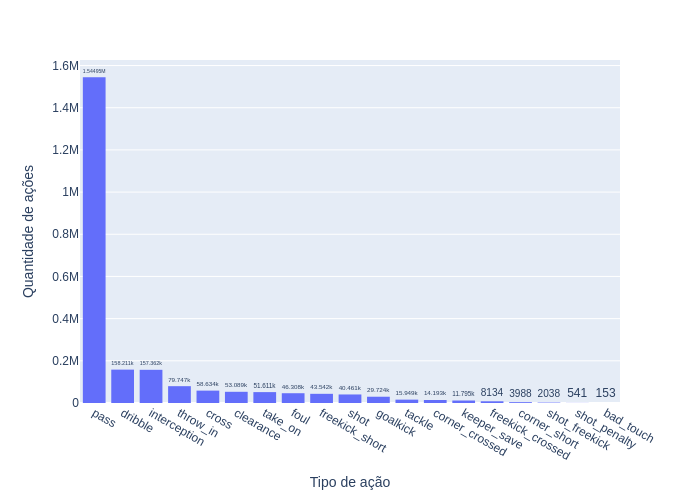
\includegraphics[width=0.8\textwidth]{images/action_distribution.png}
	\caption{Distribuições dos tipos de ação}
	\label{fig:action_distribution}
\end{figure}

\subsection{Distribuição da posição de chutes convertidos em gol}

O mapa de calor abaixo permite que sejam analisadas a distribuição das posições
dos chutes que se converteram em gol
na base de dados.

\begin{figure}[H]
	\centering
	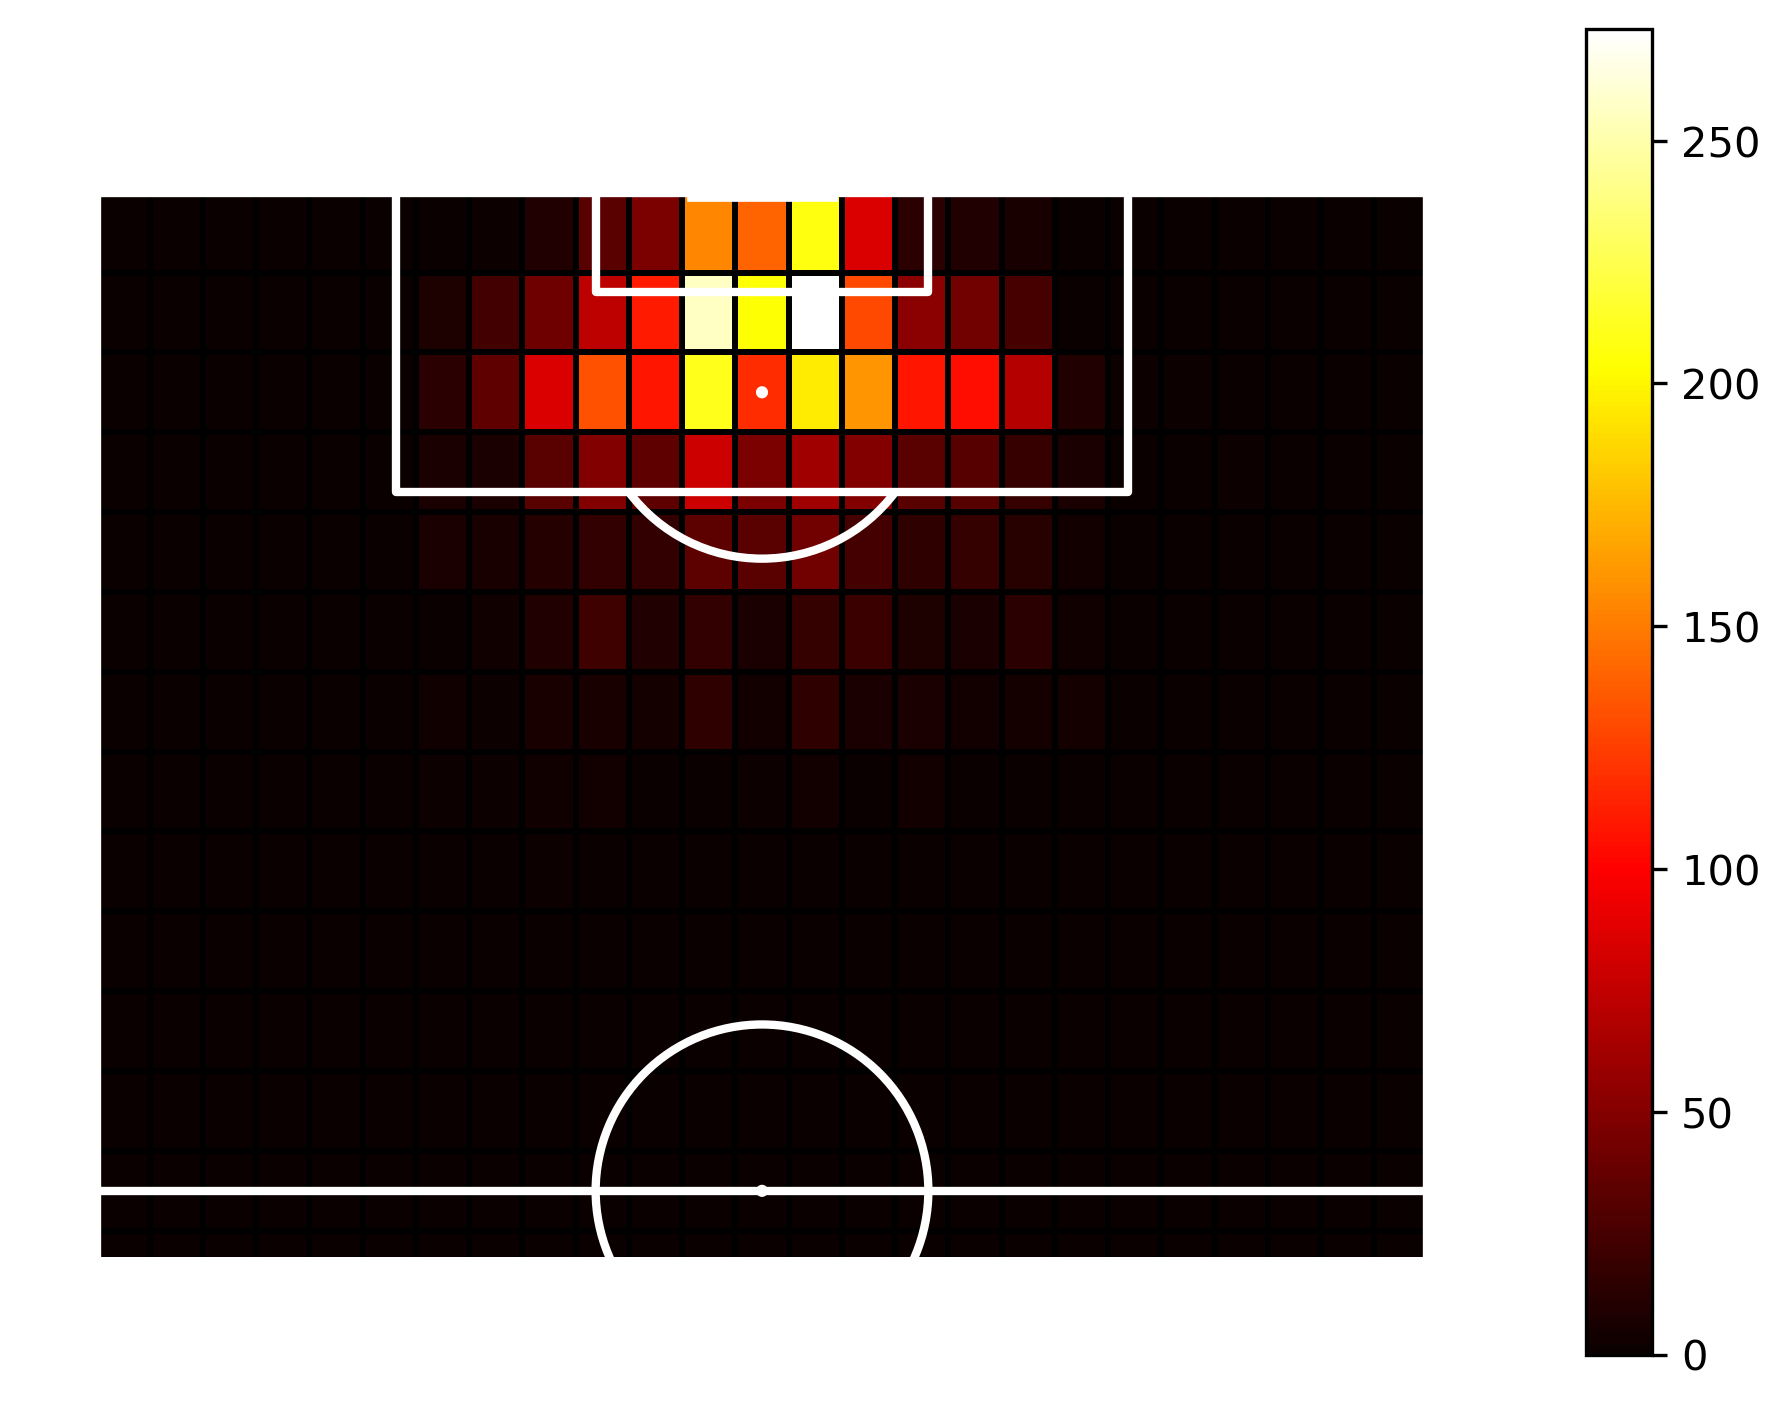
\includegraphics[width=0.5\textwidth]{images/goal_position_heatmap.png}
	\caption{Distribuições dos tipos de ação}
	\label{fig:heatmap_goals}
\end{figure}

\subsection{Distância média entre passes}

O passe é um dos, se não o fundamento mais importante em um esporte coletivo
como o futebol. Uma boa execução desse fundamento por parte dos jogadores
de uma equipe indica um bom controle da posse de bola que está diretamente
conectado com bons resultados \cite{cox2022linhas}. Nesse sentido é
interessante fazer um análise
das distâncias entre os passes
executados por cada equipe.

Em particular, foi coletada a distância entre todos os passes bem sucedidos de
cada equipe e, posteriormente, coletadas estatísticas sobre essas distâncias. A
distância média
entre passes se destacou, uma vez que ela indica como funciona a dinâmica de
troca de passes de uma equipe. Os resultados observados confirmaram suspeitas
prévias acerca do assunto.
Como pode-se notar nas tabelas abaixo, para cada uma das grandes ligas, as
principais equipes, isto é, as equipes com maior grandeza histórica e maior
poderio financeiro figuram como aquelas
que possuem a menor distância média entre passes bem sucedidos. Na Inglaterra,
por exemplo, o Manchester City, equipe comandada pelo espanhol Pep Guardiola,
foi a equipe com a menor média
de distância entre passes. O estilo de jogo de Guardiola é muito focado no
controle da posse de bola e na movimentação dos jogadores para receptar um
passe \cite{terzis2023pep}, então o resultado está dentro do
esperado.

É interessantes notar que os clubes com menor média de distância entre os
passes da temporada 17/18 em cada liga mantiveram posições altas em seus
respectivos campeonatos. O Manchester City e o Paris Saint Germain se sagraram
campeões, enquanto Napoli e Atletico de Madrid ficaram com a segunda colocação.
Na Alemanha, o RB Leipzig ficou com a sexta colocação. Pode-se notar então que
existe uma correlação entre a o desempenho de um time no campeonato com a
distância média entre os passes da equipe.

\begin{table}[H]
	\centering
	\begin{tabular}{|c|c|}
		\hline
		\textbf{Equipe}            & \textbf{Distância média entre
			passes (m)}
		\\ \hline
		Manchester City FC         & 17.208
		\\ \hline
		Arsenal FC                 & 17.729
		\\ \hline
		Manchester United FC       & 17.823
		\\ \hline
		AFC Bournemouth            & 18.417
		\\ \hline
		Tottenham Hotspur FC       & 18.490
		\\ \hline
		Crystal Palace FC          & 18.555
		\\ \hline
		Chelsea FC                 & 18.682
		\\ \hline
		Southampton FC             & 18.801
		\\ \hline
		Liverpool FC               & 18.808
		\\ \hline
		West Ham United FC         & 18.832
		\\ \hline
		Watford FC                 & 18.967
		\\ \hline
		Newcastle United FC        & 18.972
		\\ \hline
		Swansea City AFC           & 19.077
		\\ \hline
		Leicester City FC          & 19.189
		\\ \hline
		Huddersfield Town FC       & 19.215
		\\ \hline
		Stoke City FC              & 19.690
		\\ \hline
		West Bromwich Albion FC    & 19.712
		\\ \hline
		Everton FC                 & 19.785
		\\ \hline
		Brighton \& Hove Albion FC & 19.838
		\\ \hline
		Burnley FC                 & 20.634
		\\ \hline
	\end{tabular}
	\caption{Premier League}
	\label{tab:average_distance_england}
\end{table}

% Table for the Spanish League
\begin{table}[H]
	\centering
	\begin{tabular}{|c|c|}
		\hline
		\textbf{Equipe}                  & \textbf{Distância média
			entre passes
			(m)}
		\\ \hline
		Club Atlético de Madrid          & 17.581
		\\ \hline
		FC Barcelona                     & 17.618
		\\ \hline
		UD Las Palmas                    & 17.864
		\\ \hline
		Real Madrid Club de Fútbol       & 17.905
		\\ \hline
		Sevilla FC                       & 18.070
		\\ \hline
		Real Betis Balompié              & 18.659
		\\ \hline
		Villarreal Club de Fútbol        & 18.703
		\\ \hline
		Real Club Deportivo de La Coruña & 18.990
		\\ \hline
		Reial Club Deportiu Espanyol     & 19.018
		\\ \hline
		Real Sociedad de Fútbol          & 19.051
		\\ \hline
		Valencia Club de Fútbol          & 19.090
		\\ \hline
		Deportivo Alavés                 & 19.225
		\\ \hline
		Real Club Celta de Vigo          & 19.324
		\\ \hline
		CD Leganés                       & 19.340
		\\ \hline
		Levante UD                       & 19.353
		\\ \hline
		Málaga Club de Fútbol            & 19.527
		\\ \hline
		Girona FC                        & 20.133
		\\ \hline
		Athletic Club Bilbao             & 20.137
		\\ \hline
		Getafe Club de Fútbol            & 20.608
		\\ \hline
		SD Eibar                         & 20.982
		\\ \hline
	\end{tabular}
	\caption{La Liga}
	\label{tab:average_distance_spain}
\end{table}

% Table for the French League
\begin{table}[H]
	\centering
	\begin{tabular}{|c|c|}
		\hline
		\textbf{Equipe}                          & \textbf{Distância
			média
			entre passes (m)}
		\\
		\hline
		Paris Saint-Germain FC                   & 17.205
		\\ \hline
		O.G.C. Nice Côte d'Azur                  & 17.923
		\\ \hline
		Olympique de Marseille                   & 17.977
		\\ \hline
		Lille OSC Métropole                      & 17.999
		\\ \hline
		En Avant Guingamp                        & 18.008
		\\ \hline
		AS Saint-Étienne                         & 18.320
		\\ \hline
		Olympique Lyonnais                       & 18.377
		\\ \hline
		Angers SCO                               & 18.414
		\\ \hline
		FC Nantes                                & 18.544
		\\ \hline
		Amiens SC                                & 18.570
		\\ \hline
		Espérance Sportive Troyes Aube Champagne & 18.604
		\\ \hline
		FC Girondins de Bordeaux                 & 18.621
		\\ \hline
		AS Monaco FC                             & 19.099
		\\ \hline
		Stade Rennais FC                         & 19.141
		\\ \hline
		FC Metz                                  & 19.266
		\\ \hline
		RC Strasbourg Alsace                     & 19.424
		\\ \hline
		Montpellier HSC                          & 19.592
		\\ \hline
		Toulouse FC                              & 19.677
		\\ \hline
		Stade Malherbe Caen                      & 19.805
		\\ \hline
		Dijon FCO                                & 19.913
		\\ \hline
	\end{tabular}
	\caption{Ligue 1}
	\label{tab:average_distance_france}
\end{table}

% Table for the Italian League
\begin{table}[H]
	\centering
	\begin{tabular}{|c|c|}
		\hline
		\textbf{Equipe}                        & \textbf{Distância
			média entre
			passes (m)}
		\\ \hline
		SSC Napoli                             & 16.864
		\\ \hline
		FC Internazionale Milano               & 17.370
		\\ \hline
		UC Sampdoria                           & 17.980
		\\ \hline
		AC Milan                               & 18.514
		\\ \hline
		Torino FC                              & 18.564
		\\ \hline
		Benevento Calcio                       & 18.613
		\\ \hline
		ACF Fiorentina                         & 18.654
		\\ \hline
		AC Chievo Verona                       & 18.706
		\\ \hline
		SS Lazio                               & 18.712
		\\ \hline
		Atalanta Bergamasca Calcio             & 18.757
		\\ \hline
		AS Roma                                & 18.759
		\\ \hline
		Società Polisportiva Ars et Labor 2013 & 18.763
		\\ \hline
		Genoa CFC                              & 18.890
		\\ \hline
		Cagliari Calcio                        & 18.897
		\\ \hline
		Juventus FC                            & 18.983
		\\ \hline
		Udinese Calcio                         & 19.043
		\\ \hline
		Bologna FC 1909                        & 19.056
		\\ \hline
		FC Crotone                             & 19.103
		\\ \hline
		Hellas Verona FC                       & 19.202
		\\ \hline
		US Sassuolo Calcio                     & 19.646
		\\ \hline
	\end{tabular}
	\caption{Serie A}
	\label{tab:average_distance_italy}
\end{table}

% Table for the German League

\begin{table}[H]
	\centering
	\begin{tabular}{|c|c|}
		\hline
		\textbf{Equipe}              & \textbf{Distância média entre
			passes
			(m)}
		\\
		\hline
		Rasen Ballsport Leipzig      & 18.123
		\\ \hline
		TSV Bayer 04 Leverkusen      & 18.319
		\\ \hline
		BV Borussia 09 Dortmund      & 18.386
		\\ \hline
		Borussia VfL Mönchengladbach & 18.648
		\\ \hline
		FC Bayern München            & 18.835
		\\ \hline
		TSG 1899 Hoffenheim          & 19.136
		\\ \hline
		FC Schalke 04                & 19.255
		\\ \hline
		Hannover 96                  & 19.269
		\\ \hline
		VfB Stuttgart 1893           & 19.616
		\\ \hline
		1. FC Köln                   & 19.626
		\\ \hline
		Hertha BSC                   & 19.762
		\\ \hline
		Hamburger SV                 & 19.834
		\\ \hline
		VfL Wolfsburg                & 19.836
		\\ \hline
		SV Werder Bremen             & 19.883
		\\ \hline
		1. FSV Mainz 05              & 19.884
		\\ \hline
		SC Freiburg                  & 19.904
		\\ \hline
		FC Augsburg                  & 20.228
		\\ \hline
		Eintracht Frankfurt          & 20.606
		\\ \hline
	\end{tabular}
	\caption{Bundesliga}
	\label{tab:average_distance_germany}
\end{table}

\section{Extração de features}

quais features usamos e qual target (paper original usou binario e xg, propomos
usar vaep)

\section{Descoberta de subgrupos}

sd nos dados. usar pysubgroupigual no artigo domiguel

\section{Mineração de sequências}

minerar sequencias antes de gols. nao so tipo deacao,mas pegar posição no
campo, jogadores, etc

\section{Resultados}

gfdfd

\section{Conclusão}

fefre

\newpage
\bibliographystyle{plain}
\renewcommand{\refname}{Referências Bibliográficas}
\addcontentsline{toc}{section}{Referências Bibliográficas}
\bibliography{sample}
\nocite{*}

\end{document}
